\newpage
% =========================================================
% ВАРИАНТ 13
% =========================================================

\section*{Вариант 13}

В четырёхугольник \(ABCD\) вписана окружность,
\(AB=13\), \(CD=18\).
Найдите периметр четырёхугольника \(ABCD\).

\begin{center}
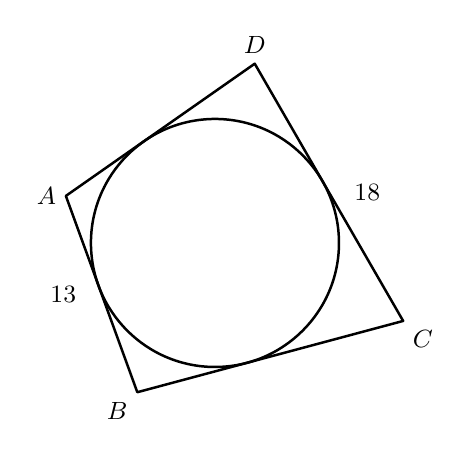
\begin{tikzpicture}[
  scale=1.05,
  line cap=round,
  line join=round,
  every node/.style={font=\small}
]
  % Координаты выбраны так, чтобы все стороны
  % четырёхугольника касались окружности радиуса 1,5.
  \coordinate (O) at (0,0);
  \coordinate (A) at (-1.803, 0.569);
  \coordinate (B) at (-0.939,-1.805);
  \coordinate (C) at ( 2.276,-0.943);
  \coordinate (D) at ( 0.481, 2.168);

  \draw[line width=0.9pt]
    (A)--(B)--(C)--(D)--cycle;

  \draw[line width=0.9pt]
    (O) circle (1.5);

  \path (A)--(B)
    node[midway,left=2mm] {$13$};

  \path (C)--(D)
    node[midway,right=2mm] {$18$};

  \node[left]        at (A) {$A$};
  \node[below left]  at (B) {$B$};
  \node[below right] at (C) {$C$};
  \node[above]       at (D) {$D$};
\end{tikzpicture}
\end{center}

\[
\boxed{\text{Ответ: }62}
\]


% =========================================================
% ВАРИАНТ 14
% =========================================================

\section*{Вариант 14}

Через концы дуги \(AB\) окружности с центром \(O\)
проведены касательные \(CA\) и \(CB\).
Угол \(CAB\) равен \(39^\circ\).
Найдите угол \(AOB\). Ответ дайте в градусах.

\begin{center}
\begin{tikzpicture}[
  scale=1.35,
  line cap=round,
  line join=round,
  every node/.style={font=\small}
]
  \def\R{1.8}
  \pgfmathsetmacro{\cx}{\R/cos(39)}

  \coordinate (O) at (0,0);
  \coordinate (A) at (39:\R);
  \coordinate (B) at (-39:\R);
  \coordinate (C) at (\cx,0);

  % Окружность
  \draw[line width=0.9pt] (O) circle (\R);

  % Касательные и хорда
  \draw[line width=0.9pt] (C)--(A);
  \draw[line width=0.9pt] (C)--(B);
  \draw[line width=0.9pt] (A)--(B);

  % Радиусы
  \draw[line width=0.75pt] (O)--(A);
  \draw[line width=0.75pt] (O)--(B);

  % Прямые углы при точках касания
  \pic[
    draw,
    line width=0.6pt,
    angle radius=3mm
  ] {right angle=O--A--C};

  \pic[
    draw,
    line width=0.6pt,
    angle radius=3mm
  ] {right angle=C--B--O};

  % Данный угол
  \pic[
    draw,
    line width=0.65pt,
    angle radius=5mm
  ] {angle=B--A--C};

  \node at (1.63,0.52) {$39^\circ$};

  \fill (O) circle (1.2pt);

  \node[left]        at (O) {$O$};
  \node[above right] at (A) {$A$};
  \node[below right] at (B) {$B$};
  \node[right]       at (C) {$C$};
\end{tikzpicture}
\end{center}

\[
\boxed{\text{Ответ: }78}
\]


% =========================================================
% ВАРИАНТ 15
% =========================================================

\newpage

\section*{Вариант 15}

Четырёхугольник \(ABCD\) вписан в окружность.
Угол \(ABC\) равен \(106^\circ\), угол \(CAD\) равен \(69^\circ\).
Найдите угол \(ABD\). Ответ дайте в градусах.

\begin{center}
\begin{tikzpicture}[
  scale=1.15,
  line cap=round,
  line join=round,
  every node/.style={font=\small}
]
  \def\R{2.3}

  \coordinate (O) at (0,0);
  \coordinate (A) at (200:\R);
  \coordinate (B) at (140:\R);
  \coordinate (C) at (52:\R);
  \coordinate (D) at (274:\R);

  % Окружность
  \draw[line width=0.9pt] (O) circle (\R);

  % Вписанный четырёхугольник
  \draw[line width=0.9pt]
    (A)--(B)--(C)--(D)--cycle;

  % Диагонали, необходимые для углов CAD и ABD
  \draw[line width=0.8pt] (A)--(C);
  \draw[line width=0.8pt] (B)--(D);

  % Угол ABC
  \pic[
    draw,
    line width=0.65pt,
    angle radius=5mm
  ] {angle=A--B--C};

  % Угол CAD
  \pic[
    draw,
    line width=0.65pt,
    angle radius=5mm
  ] {angle=D--A--C};

  \node at (-1.05,1.15) {$106^\circ$};
  \node at (-1.38,-0.62) {$69^\circ$};

  \node[left]        at (A) {$A$};
  \node[above left]  at (B) {$B$};
  \node[above right] at (C) {$C$};
  \node[below]       at (D) {$D$};
\end{tikzpicture}
\end{center}

\[
\boxed{\text{Ответ: }37}
\]


% =========================================================
% ВАРИАНТ 16
% =========================================================

\section*{Вариант 16}

Четырёхугольник \(ABCD\) вписан в окружность.
Угол \(BAD\) равен \(127^\circ\).
Найдите угол \(BCD\). Ответ дайте в градусах.

\begin{center}
\begin{tikzpicture}[
  scale=1.15,
  line cap=round,
  line join=round,
  every node/.style={font=\small}
]
  \def\R{2.3}

  \coordinate (O) at (0,0);
  \coordinate (A) at (190:\R);
  \coordinate (B) at (130:\R);
  \coordinate (C) at (0:\R);
  \coordinate (D) at (236:\R);

  \draw[line width=0.9pt] (O) circle (\R);

  \draw[line width=0.9pt]
    (A)--(B)--(C)--(D)--cycle;

  \pic[
    draw,
    line width=0.65pt,
    angle radius=5mm
  ] {angle=D--A--B};

  \node at (-1.37,-0.10) {$127^\circ$};

  \node[left]        at (A) {$A$};
  \node[above left]  at (B) {$B$};
  \node[right]       at (C) {$C$};
  \node[below left]  at (D) {$D$};
\end{tikzpicture}
\end{center}

\[
\boxed{\text{Ответ: }53}
\]


% =========================================================
% ВАРИАНТ 17
% =========================================================

\newpage

\section*{Вариант 17}

Градусная мера дуги \(AB\) окружности, не содержащей точку \(D\),
равна \(106^\circ\).
Градусная мера дуги \(DE\) окружности, не содержащей точку \(A\),
равна \(48^\circ\).
Найдите угол \(ACB\). Ответ дайте в градусах.

\begin{center}
\begin{tikzpicture}[
  scale=1.05,
  line cap=round,
  line join=round,
  every node/.style={font=\small}
]
  \coordinate (O) at (0,0);

  % Точки на окружности радиуса 2
  \coordinate (A) at (0,-2);
  \coordinate (B) at (-1.923,0.551);
  \coordinate (D) at (1,1.732);
  \coordinate (E) at (1.956,0.416);

  % Внешняя точка пересечения секущих
  \coordinate (C) at (4.005,2.946);

  \draw[line width=0.9pt] (O) circle (2);

  % Секущие CDB и CEA
  \draw[line width=0.9pt] (C)--(B);
  \draw[line width=0.9pt] (C)--(A);

  % Обозначение внешнего угла
  \pic[
    draw,
    line width=0.65pt,
    angle radius=5mm
  ] {angle=B--C--A};

  % Подписи градусных мер дуг
  \node at (218:2.42) {$106^\circ$};
  \node at (36:2.42) {$48^\circ$};

  \fill (A) circle (1.1pt);
  \fill (B) circle (1.1pt);
  \fill (D) circle (1.1pt);
  \fill (E) circle (1.1pt);

  \node[below]       at (A) {$A$};
  \node[left]        at (B) {$B$};
  \node[above]       at (D) {$D$};
  \node[below right] at (E) {$E$};
  \node[above right] at (C) {$C$};
\end{tikzpicture}
\end{center}

\[
\boxed{\text{Ответ: }29}
\]


% =========================================================
% ВАРИАНТ 18
% =========================================================

\section*{Вариант 18}

Радиус окружности, описанной около треугольника \(ABC\),
равен \(2\sqrt3\).
Найдите \(AB\), если угол \(ACB\) равен \(120^\circ\).

\begin{center}
\begin{tikzpicture}[
  scale=1.15,
  line cap=round,
  line join=round,
  every node/.style={font=\small}
]
  \def\R{2.3}

  \coordinate (O) at (0,0);
  \coordinate (A) at (150:\R);
  \coordinate (B) at (30:\R);
  \coordinate (C) at (90:\R);

  \draw[line width=0.9pt] (O) circle (\R);

  \draw[line width=0.9pt]
    (A)--(B)--(C)--cycle;

  \pic[
    draw,
    line width=0.65pt,
    angle radius=5mm
  ] {angle=A--C--B};

  \node at (0,1.40) {$120^\circ$};

  \node[left]        at (A) {$A$};
  \node[right]       at (B) {$B$};
  \node[above]       at (C) {$C$};

  \node[below] at (0,-2.45) {$R=2\sqrt3$};
\end{tikzpicture}
\end{center}

\[
\boxed{\text{Ответ: }6}
\]



\end{document}